\section {Shape Detection}
\label{sec:related_work_shape detection}

The objective of detecting structures in point clouds is a wide field of research. The term structure is very loosely defined. Structure can mean geometric structures, such as planes, cylinder, or spheres. Structure can also be interpreted as more complex components that represent distinct man-made or natural formations, such as cars or lanterns. 
\\
The 2D Hough transform \cite{hough1962method} is a technique usually used in the field of image processing. This method can detect straight lines such as building contours as well as curves. When extending the Hough transform to 3D by Maas et al. \cite{maas1999two} and later by Oda et al. \cite{oda2004automatic} and Overby et al. \cite{overby2004automatic}, the technique can detect planes and other geometric forms such as cylinders \cite{rabbani2005efficient}. 

\begin{figure}
    \centering
    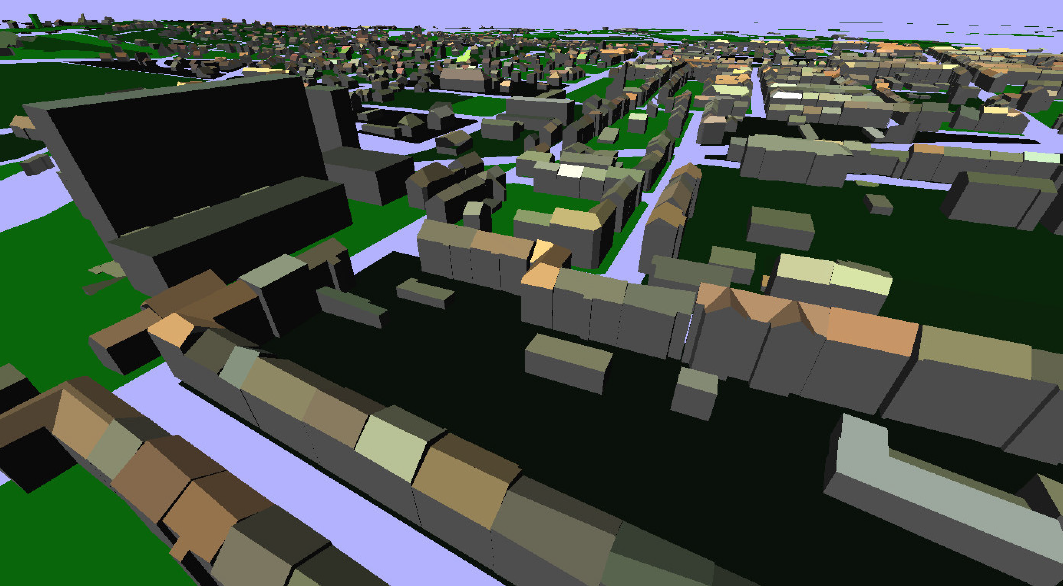
\includegraphics[width=0.81\textwidth]{Related_Work/hough_planes.png}%7
    \caption[Scene created by using 3d Hough transform to detect planes from an airborne laser scanner]
		{Scene created by using 3d Hough transform to detect planes from an airborne laser scanner. Image by Overby et al. \cite{overby2004automatic}.}
    \label{fig:hough_planes}
\end{figure}

Figure \ref{fig:hough_planes} shows a city model consisting of planes, detected using 3d Hough transform, in a point cloud obtained from airborne laser scanning. Figure \ref{fig:hough_cylinder} showcases a point cloud obtained by a 3d scan and the detected cylinder. 


\begin{figure}
\centering
\subcaptionbox{ \label{fig:picking_raycast }}{
  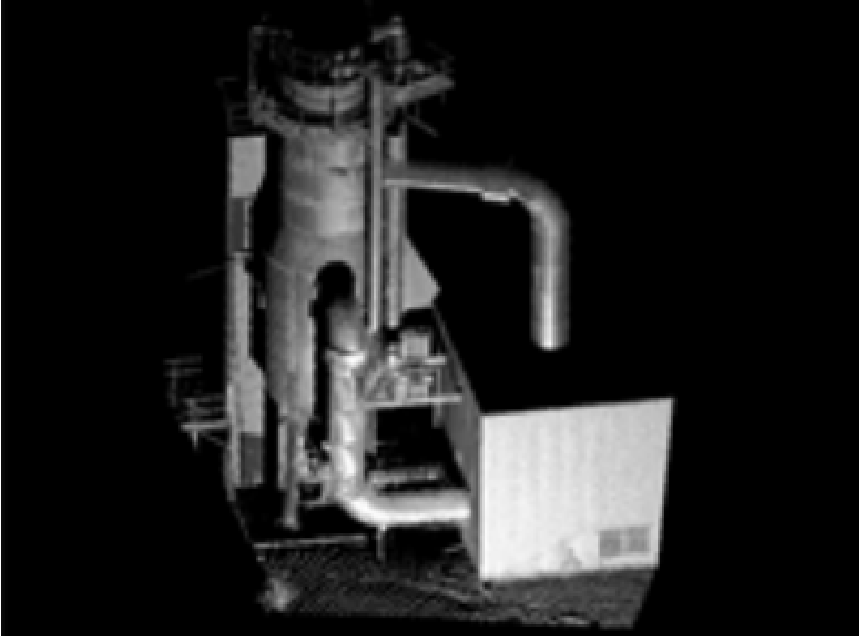
\includegraphics[width=0.4\textwidth]{Related_Work/hough_cylinder1.png}
  }
\subcaptionbox{ \label{fig:picking_conecast }}{
  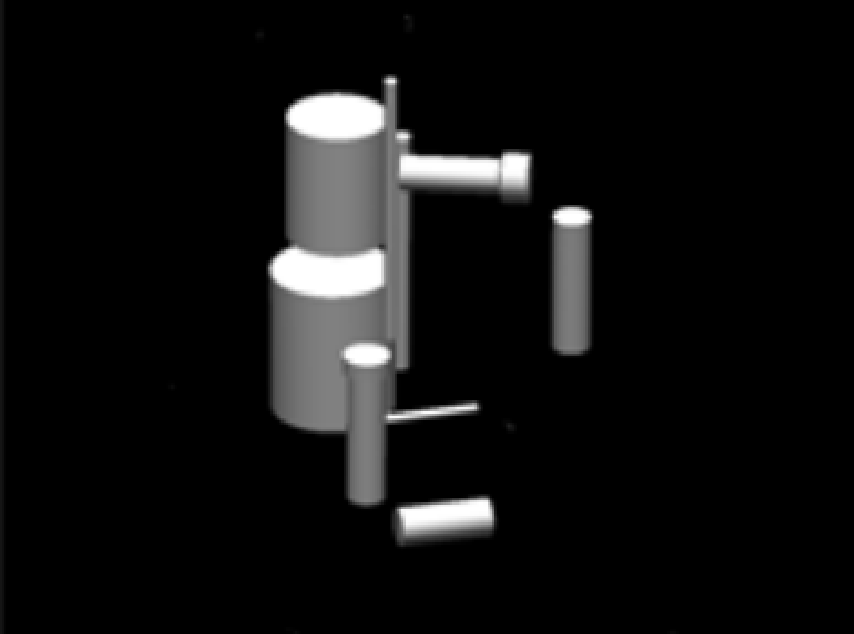
\includegraphics[width=0.4\textwidth]{Related_Work/hough_cylinder2.png}
  }
\caption[Results of 3d Hough transform used to detect cylinder]
{This figure shows the results of 3d Hough transform used to detect cylinder. (a) shows the input point cloud, (b) shows the detected cylinder. Image by Rabbani et al. \cite{rabbani2005efficient}.}
\label{fig:hough_cylinder}
\end{figure}


A more recent approach by Schnabel et al. \cite{schnabel-2007-efficient} utilizes Random Sampling Consens \cite{fischler1981random} to extract a minimal set of primitive shapes that approximate the global structure of the point cloud. The algorithm randomly selects a set of points that roughly follow the curvature of a shape. If a defined number of points follow this shape's curvature as well, the shape is considered to be valid. This approach is capable of detecting planes, cylinders, spheres, cones, and tori and has evolved into one of the most prominent shape detection algorithms and is used in this thesis as well. 

\begin{figure}
    \centering
    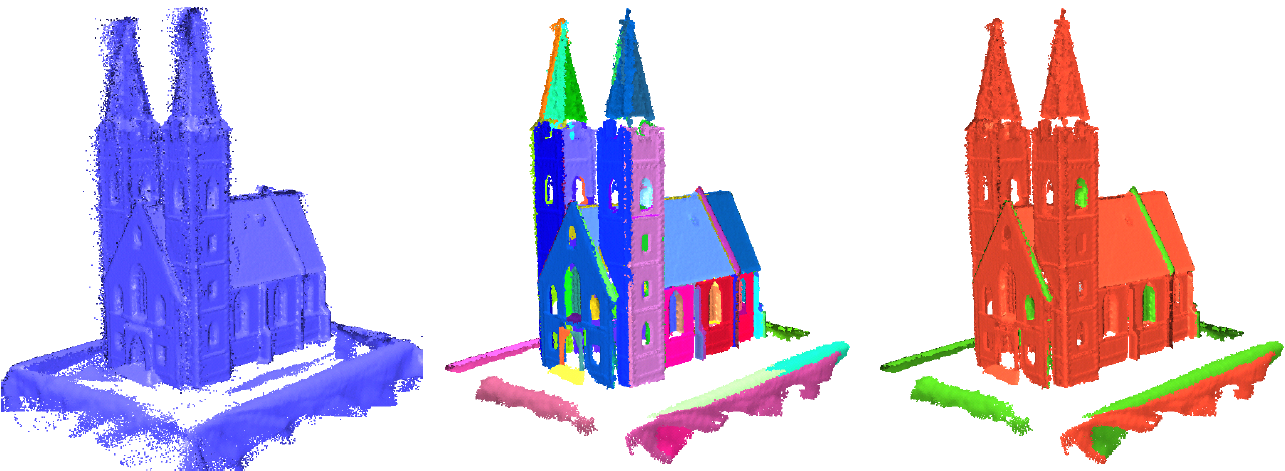
\includegraphics[width=0.8\textwidth]{Related_Work/schnabel_example.png}%7
    \caption[Church with points colored by detected shape]
		{Left: the original point cloud. Center: The points that belong to a detected shape in random colors. Right: The colors are determined by type (plane = red, cylinder = green, sphere = yellow, cone = purple, torus = grey). Image by Schnabel et al. \cite{schnabel-2007-efficient}. }
    \label{fig:schnabel_church}
\end{figure}

Figure \ref{fig:schnabel_church} shows the results of the RANSAC approach on a point cloud. Not only does this approach provide the geometry of the detected shapes, it also determines the membership of a point to a shape. 
\\
\\
Tarsha-Kurdi \cite{tarsha2007hough} analyzes the performance of the 3D Hough transform and RANSAC for detecting roof planes from airborne laser data. RANSAC proves to be more robust to noise and more efficient.
\\
\\
GlobFit is a system by Li et al. \cite{li2011globfit} that aims to recover a set of locally fitted primitives, obtained by RANSAC, along with their global mutual relations. The authors work under the assumption that primitives occur repeatedly and are man-made, so global relations are iteratively learned and enforced on the local relations. 
\\
\\
Golvinskiy et al. \cite{golovinskiy2009shape} utilize graph-based methods to recognize shapes in urban environments in 3D point clouds. This method can detect objects, such as cars, newspaper boxes and traffic lights. Potential object locations are identified by clustering nearby points before the point cloud is segmented into foreground and background. For each cluster, a feature vector is built, before using it as input for a trained classifier to obtain a final classification. 
\\
\\
Oesau et al. \cite{oesau2016planar} propose an alternative approach to detect planar shapes in point clouds by using region growing. A shape is represented as a set of points and an associated fitting plane. Points or shapes from the neighborhood are added consecutively to the plane, thus growing the region. 